\chapter{Fetch Stage}

We are ready to build our fetch unit.  To do this, we will make one more unit, our instruction memory, then we will need to make a module to assemble all our units together.


\section{Instruction Memory}
The instructions are stored in memory, and are accessed by using the address where they are stored.  You can think of memory like a giant hotel for our data.  Each piece of data is an integer, and gets stored in a room (memory location), which we can find by its room number (memory address).  To get a piece of data, like an instruction, stored in memory we need to take its address, go to that location, and grab the value.  A bunch of memory locations, accessed by an address is called an array.  Arrays are declared like they are in C; the data type is specified, then the name, then the array size.  To store the instructions, we will need an array of 32-bit numbers (definitions.vh defines INSTR\_LEN as 32), which means the data type must be \verb2reg[`INSTR_LEN-1:0]2.  After the name is specified (mem in this case), we are going to use a parameter called SIZE to specify how big the array is: \verb2[SIZE-1:0]2.

The other interesting thing about this code is how to initialize the memory.  The default size of the memory is 4KB, which is impractical to setup using for loops and such, so we read it from memory.  Fortunately Verilog gives you two functions to do this automatically: \$readmemb and \$readmemh.  The last letter specifies the base (binary or hexadecimal) of the data in the file.  White space separates fields, but the underscore character is ignored and thus can be used to make the values in a number more readable.

\Verilog{Instruction Memory}{code:instmem}{../code/1_fetch/instr_mem.v}

The code is given in Listing~\ref{code:instmem}.  What needs to be tested?  How will it be used?  What can go wrong?  Consider those questions and write a testbench and verify it's operation.

\section{Fetch Stage}
Now we need to connect it together.  The components of our instruction fetch (sometimes called ifetch or just fetch) stage are shown in Figure~\ref{fig:fetch}.

\begin{wrapfigure}{L}{2in}
\caption{Instruction Fetch Stage.}\label{fig:fetch}
\begin{center}
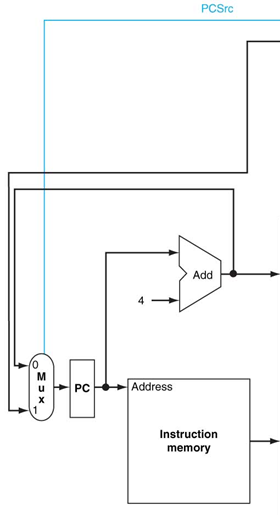
\includegraphics[width=2in]{../images/pipeline_fetch.png}
\end{center}
\end{wrapfigure}

Any wire (or reg) in the figure that comes in or goes out are ports.  In Figure~\ref{fig:fetch}, the blue wire is a control signal and comes ultimately from the control unit, which you will build in the next stage called decode.   Wires (or regs) that are completely contained in the figure are local and are thus defined in the module.  This is important to notice when setting up your own modules, so try to figure out which each is before looking at the starter code.  Equally important is determining the size of each signal (wire or reg), and following the convention (big or little endian).  When you look at the figure I cut from a figure in the book, note that not every wire has a name.  If a wire is unlabeled it is worth looking at other figures (like your text in chapter 4) to get the names.  In some cases the names don't matter, so a suitable name, that expresses the signal identity, location, and/or use is advisable.  One nice convention\footnote{Other conventions to consider are: CamelCase, underscore\_separation.  I honestly mix them when I am doing small projects or when I want to expose students to both, but in a formal design you should pick one and stick with it.  Mistyping a variable is a frequent, and annoying, source of errors.} I have used at times would label the program counter signal in the fetch stage as \verb1PC_fetch1.  Similarly the next program counter signal passed from fetch to decode would be \verb1nPC_fetch-decode1.  Note you get directionality also.  Sometimes this helps, sometimes it is cumbersome, it mainly helps in debugging and modifying.  Good names are slower now when it is easy (setup), and faster later when it is hard (debug), and is one of my favorite take-aways from the Agile design method called extreme programming.  Most people are in a rush to get something done, so they make the design impossible - don't fall in this trap!

Once you have figured out all your connecting signals (wires and regs), you should identify the components you are going to use.  We have already created the modules, so now we just need to tell Verilog to instantiate them (build one).  Again choose your names wisely.  I have instantiated for you, but I don't have my connections done.  Well I have one, and that is because it is a tricky one.  An output in Verilog cannot be read inside the module that creates it.  In our case nPC must be an output, but also needs to be read internally.  I handle this by creating a local wire that can be read and assigning its value to the output.  I thought this would be sneaky at the start so I wired it up.  You must use the wiring diagram to hook the components together with the available wires.

The code, minus the connections is listed below in Listing~\ref{code:fetch}.  Once you have done your connections you should test how well the code works.  You will only be able to see nPC and instruction coming out, so think how you can simulate the behavior of a computer, and what you should check.  You know you checked your individual modules, but there could be errors, or unexpected behavior.  Sometimes weird timings between modules causes signals to be missed and such.  Think about what could happen and how you would have to recover (use of reset).  Test sequential and branching.  You can break your tests into several small tests too, which is often easier.  Calling them something like ``iFetch\_test\_sequential.v'' to distinguish the contents is helpful later.

\Verilog{Starter code for the fetch stage.}{code:fetch}{../code/1_fetch/iFetch.v}

\section{Your Assignment}
You are to:
\begin{enumerate}
\item Write a testbench for the memory in Listing~\ref{code:instmem}.
\item Finish the fetch stage and write a testbench to verify it.
\item Run the simulations and generate a timing diagrams.
\item  Write up a lab report in \LaTeX\ following the lab format in \verb1LabN.tex1 and generate a pdf file.
\item Upload the pdf and all the Verilog files to the course LMS.
\end{enumerate} 